\documentclass[12pt,titlepage,oneside]{book}
\usepackage[T1]{fontenc} % modern encoding
% Comment out the next three lines of LaTeX if you wish to use Computer Modern fonts
%   (this is the default for LaTeX)
% Make sure that your TeX installation can produce good pdf with these fonts.
% The following three lines are a good alternative if you don't use much mathematics
\usepackage{mathptmx}  % uses Times for text and mathematics
\usepackage[scaled]{helvet} %  helvetica for sanserif, scaled 95% by default
\usepackage{courier}  % courier for typewriter font, pretty ugly but available
% otherwise the stix package offers more options and symbols
% \usepackage{stix}  % uses Times for text and a range of fonts for mathematics
% End of choices for fonts
\usepackage{graphicx}  % standard package for importing graphics files
%\usepackage{cite}  % improves format of numerical citations, such as [1-3]
\usepackage[top=2.5cm, bottom=1.5cm,left=2.5cm,right=2.0cm]{geometry}
% These margins are the university guidelines
\usepackage[onehalfspacing]{setspace}  % gives one-and-a-half line spacing
% doublespacing is another option and can be changed in the text

% My packages:
\usepackage{titling}
\usepackage[british]{babel}
\usepackage[outputdir=build]{minted}
\usepackage{listings}
\usepackage{siunitx}
\usepackage{nameref}
\usepackage{enumitem}
\usepackage[useregional]{datetime2}
\usepackage{enumitem}
\usepackage[round,authoryear]{natbib}

\usepackage[super]{nth}
\usepackage{hyperref}

% Settings
%\inputminted[breaklines]{cpp} %fontsize=\footnotesize,
\DTMlangsetup[en-GB]{showdayofmonth=false}

\setcounter{tocdepth}{2}

\title{MSc Project: Oscillometric Blood Pressure}
\author{Belinda Kneubuhler}
\date{\today}

\newcommand*{\myref}[1]{\ref{#1}~\nameref{#1}}%#todo fix:
\newcommand{\stdNbr}{2504756K}
\newcommand{\course}{MSc Computer Systems Engineering}

\begin{document}

% Settings:
\lstset{language=C++}
\sisetup{range-units=single}

\begin{titlepage}
\centering
%\vspace*{3cm}  % Need the * or the space is swallowed at the top of the page


\includegraphics[scale=0.125]{GlaLogo.pdf}\\
\vspace{1cm}
\bfseries\Large
\thetitle\\

%TODO add a picture here

\vspace*{\fill}
\begin{tabular}{c c}
Belinda Kneubühler & \stdNbr\\
\end{tabular}

\normalfont\large
\vspace{1cm}
School of Engineering\\
College of Science and Engineering\\
University of Glasgow\\

\vspace{1cm}
Submitted in fulfilment of the requirements for the\\
Degree of \course\\
\vspace{1cm}
\begin{flushleft}
\begin{tabular}{l r}
Supervisor: & Bernd Porr\\
Second Supervisor: & Kiran Ramesh\\
\end{tabular}
\end{flushleft}

% Insert month and year of date deposited with library for final version
\thedate

\end{titlepage}
\frontmatter  % Turn off chapter numbering, use roman page numbers
\chapter{Abstract}

Abstract text goes here.

\tableofcontents
\listoftables
\begingroup
\let\clearpage\relax
\listoffigures
\endgroup
\chapter{Acknowledgements}

Acknowledgements text goes here.

\chapter{Declaration}
%TODO update at the end
%With the exception of chapters 1, 2 and 3, which contain introductory material, all work in this thesis was carried out by the author unless otherwise explicitly stated.


\mainmatter % Turn on chapter numbering, reset page numbers, use arabic
\chapter{Introduction}

\begin{figure}
\centering

\includegraphics[scale=0.125]{GlaLogo.pdf}
\caption{This is the university logo, used as an example because it is needed for the front page.}
\label{logo figure}
\end{figure}

Here starts the thesis with some text to check that things are working. Let's refer to figure \ref{logo figure} to check that the captions and labels work. I shall also check that \textsf{sanserif} and \texttt{typewriter} work. And here is equation (\ref{inductor iv}) too,
\begin{equation}
v = L \frac{di}{dt} .
\label{inductor iv}
\end{equation}
A report is a formal document and should be written in appropriate language. Numerous books offer advice on writing reports and a selection is listed in the references at the end. Here are a few tips.
\begin{itemize}
\item
Reports should be written in correct English. Break text into paragraphs, keep sentences to a reasonable length and insert appropriate punctuation. Use a spell-checker and a grammar-checker if desired but neither is a substitute for careful reading.
\item
A report is not a story.
Write `The voltage was measured' rather than `I measured the voltage'. This document contains instructions and therefore uses a different style.
\item
Define all abbreviations when they are first used: `The accelerometer uses a serial peripheral interface (SPI)'. Provide a list of abbreviations if you use a large number of them.
\item
Don't write material that you don't understand. It will be obvious to the reader.
\end{itemize}
The quality of English is assessed as part of the report. Foreign students may feel this to be a burden but part of their education in this country is to learn to work effectively in an English-speaking environment. \cite{Geddes1982}


\section{Precision}

An engineering report must be precise. This applies both to the language and to numerical values. For example, the words \emph{precision} and \emph{accuracy} are often used interchangably in non-technical discussion but the distinction between them is vital in engineering. Vague, waffly text is a major weakness of many students' technical reports (and examination answers).

\subsection{A subsection}

Figures (diagrams, photographs etc) and tables must have informative captions and be numbered. Axes of graphs should have scales, titles and units, otherwise the plot is meaningless. Multiple curves must be labelled, either directly or with a caption. Use dotted or dashed lines as well as colour for clarity; remember that the reader might be colour-blind or have only a black-and-white printout. All text must be legible, roughly the same size as the main text. Be warned that plots from Excel or Matlab need extensive editing to bring them up to an acceptable standard. Experimental traces can be captured on most modern test equipment and can make good illustrations.

\chapter{Theory}\label{cp:theory} %TODO maybe call this chapter background
This chapter discusses the findings of researching existing and proposed algorithms for determining systolic and diastolic blood pressure through the oscillometric method.

The method was described and tested by Geddes et al. in 1982 \cite{Geddes1982}. The mean arterial pressure (MAP) is generally described as the pressure at which oscillation amplitudes are maximal. Geddes is determining ratios of the MAP to find the systolic and diastolic blood pressure. He defines the ratio for the systolic pressure to be 0.5 and the ratio for the diastolic pulse as 0.8. These ratios were found in an experimental way and Geddes acknowledges that the systolic pressure is overestimated and the ratio for the diastolic pulse is not constant for a range of different diastolic pressures.

Later studies tried to find accurate ratios, mostly experimentally. Mathematical models confirmed that a generalised ratio cannot be found. Parameters like the age of the subject and in this regard, the arterial stiffness influence the ratios. \cite{Babbs2012}

\chapter{Algorithm}\label{cp:algo}

This chapter explains the general principles behind the algorithm and separates the logic from the implementation, which will be discussed in a separate chapter, \nameref{cp:sw}. 

The realised algorithm is a fixed-ratio algorithm. It analyses the oscillations to find MAP form the maximum amplitude as described in \myref{sec:MAA} and estimates the position of the systolic and diastolic BP as where the amplitudes are at a specific ratio of the maximum. The systolic BP is evaluated while the oscillation amplitudes increase and the diastolic BP while they decrease, respectively.


\begin{figure}[ht]
\centering
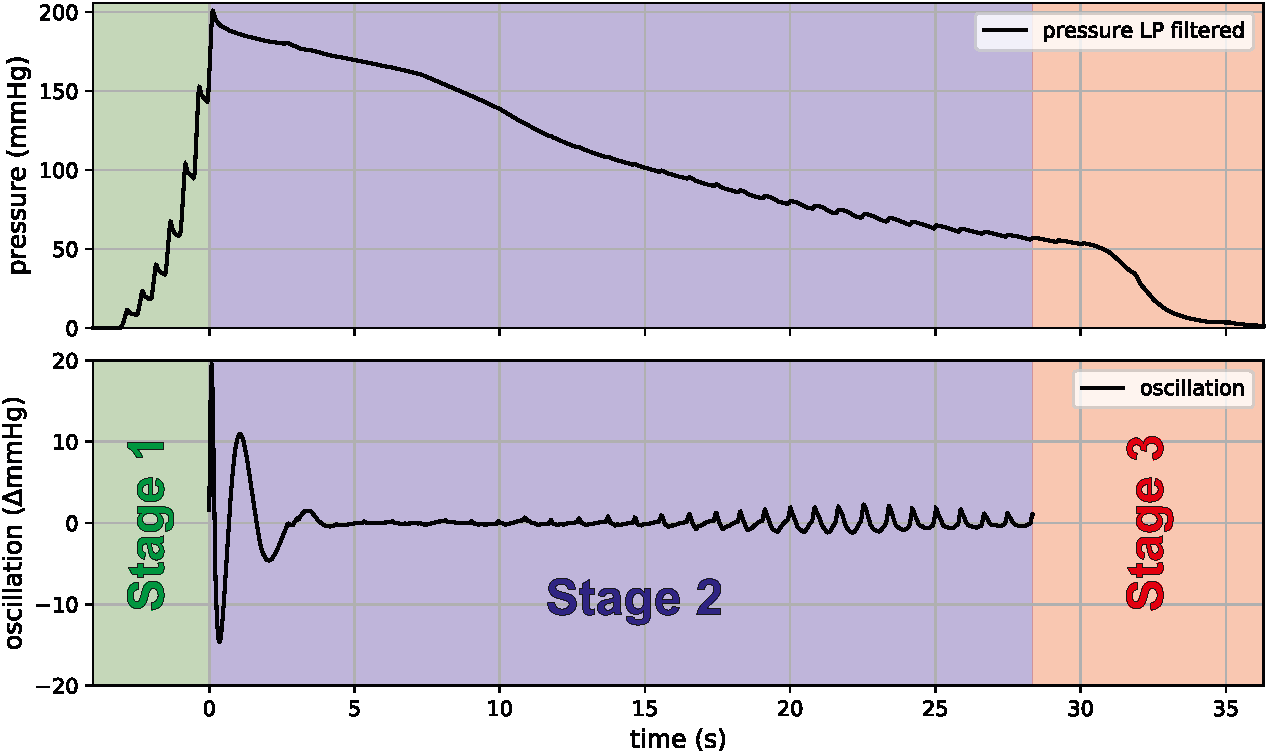
\includegraphics[width=\textwidth]{figures/algo_overview.pdf}
\caption{A sample data set is shown in the top plot and divided into three parts. The blue part is where oscillations are analysed. These are shown in the bottom plot.}
\label{fig:algoOverview}
\end{figure}

The top plot in figure \ref{fig:algoOverview} shows one data set and how it is divided into different steps for processing. The first part (green) is when the user pumps up the cuff pressure. The second part (blue) is the deflation. Here, the oscillations, shown in the bottom plot, are recorded and analysed. Once these oscillations have increased to a maximum and decreased again to a certain value, the last step (red) is simply the deflation of the cuff. The core part of the algorithm works on the blue part of the data.



\section{Preprocessing}
The data is always filtered. Additionally, preprocessing decides which stage of the dataset is active. In relation to figure \ref{fig:algoOverview} stage one is green, stage two is blue and stage three is red. Figure \ref{fig:stage1} shows the basic diagram of the data processing. Only the deflating and filtered data is processed by the core algorithm. 

\subsection{Filtering}\label{sec:filt}
To remove unwanted noise from the data and to get the oscillations, two filters are used. Figure \ref{fig:stage1} shows the simple cascade of a low-pass (LP) and high-pass (HP) filter, resulting in a bandpass(BP) filtered output signal, the oscillogram. The results of both filter outputs are used in the algorithm.
%
%\begin{figure}[ht]
%\centering
%\includegraphics[width=0.7\textwidth]{figures/filter_cascade.pdf}
%\caption{The simple basic data processing flow. The data is acquired and passed first to a low-pass filter \SI{10}{\Hz} and then to a high-pass filter of \SI{0.5}{\Hz}, resulting in a bandpass output.}
%\label{fig:filter_cascade}
%\end{figure}

\begin{figure}[ht]
\centering
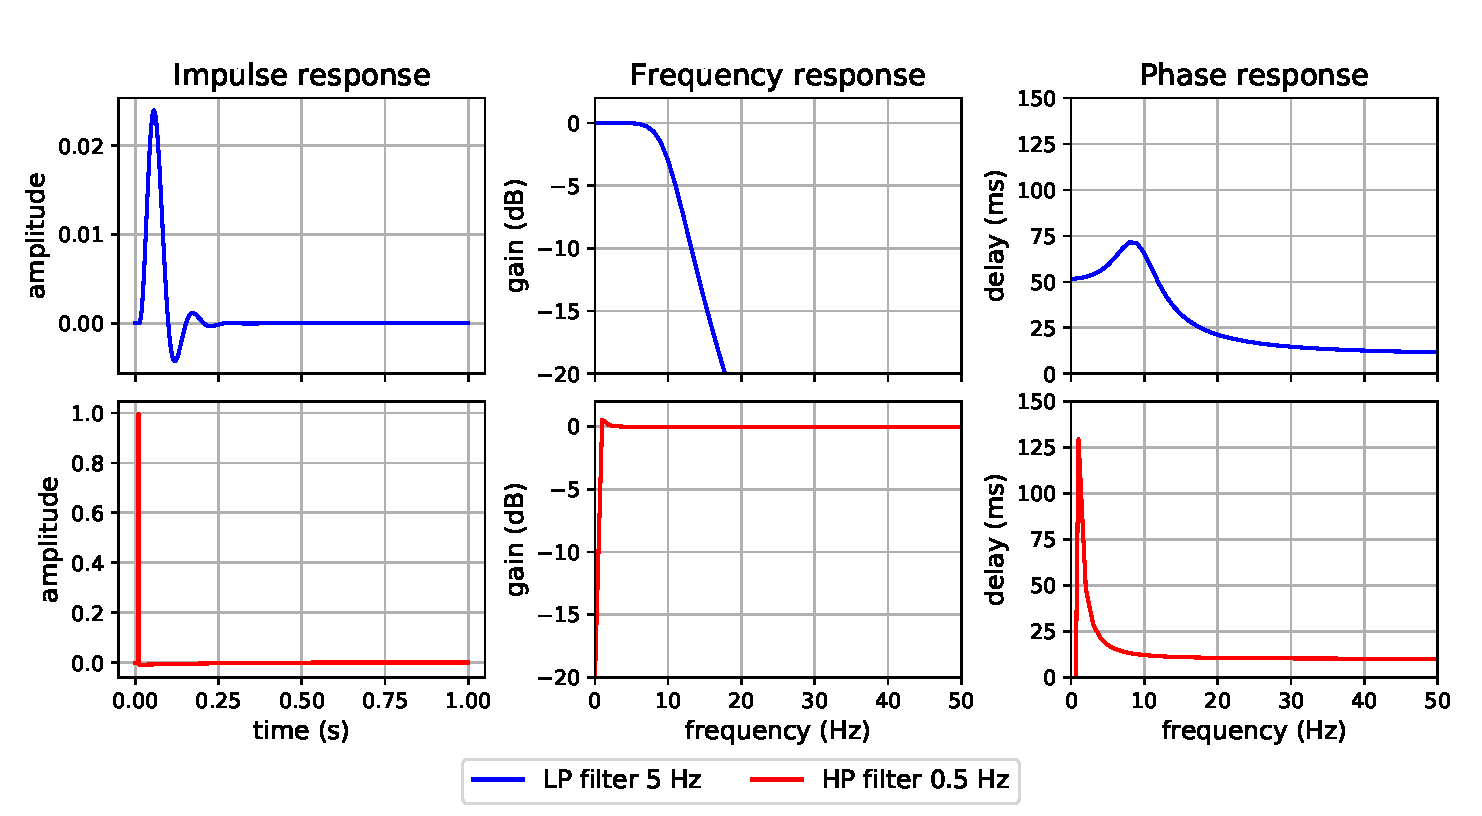
\includegraphics[width=\textwidth]{figures/filter.pdf}
\caption{Filter.}
\label{fig:filters}
\end{figure}
%All data is filtered. 

From the research done in chapter \ref{cp:theory}, it is known that most algorithms use band pass filters of low orders up to \nth{6} and with cut-off frequencies between \SIrange{0.1}{0.5}{\Hz} and \SIrange{5}{20}{\Hz} \citep{Forouzanfar2015}. The implemented algorithm does not rely on pulse shape and can therefore use relaxed constraints. Best results were achieved with a lower cut-off frequency of \SI{0.5}{\Hz}. The upper cut-off frequency was fixed \SI{10}{\Hz}. Generally, there is very little activity between \SIrange{5}{20}{\Hz}, but because no experiments could be made, a mean value was chosen. 

The implemented filters are shown in figure \ref{fig:filters}. The low-pass filter has a small delay in the impulse response and the phase response shows that for very low frequencies there is a slightly higher delay. The frequency response shows a steep slope after \SI{10}{\Hz} and suppression of more than \SI{20}{\decibel} of every frequency above \SI{20}{\Hz}. The HP filter expectedly lets the impulse pass. In the frequency response there is a small overshoot but otherwise a good suppression of DC. The bottom left plot in figure \ref{fig:filters} shows that HP filter has a significantly delay of about \SI{125}{\milli\second} for frequencies around \SI{1}{\Hz}. This could potentially cause inaccuracies. Section \ref{sec:impfilt} will show, why this is not a problem.


%TODO referecne section


\subsection{Stage Detection}
The LP filtered data is analysed by the preprocessing step to detect if the second stage, the deflation, is active. Figure \ref{fig:stage1} shows how the preprocessing step then passes both the LP and BP filtered data to the core algorithm, symbolised by a switch. 

In the first stage, the data is checked if the pressure in the cuff is high enough to start deflation and if so, the preprocessing switches to the second stage. This value is configurable. The default value is \SI{180}{\mmHg}. Figure \ref{fig:stage1} shows how the decision is made based on the LP filtered data.  

Once the second stage is active, the preprocessing checks the core algorithm if it is done. In figure \ref{fig:stage1} this is indicated by the arrow from the algorithm back to preprocessing. Additionally, the data is checked if it is below a value of \SI{20}{\mmHg}, where blood pressure measurements make no sense, and the measurement is  potentially cancelled.

\begin{figure}[ht]
\centering
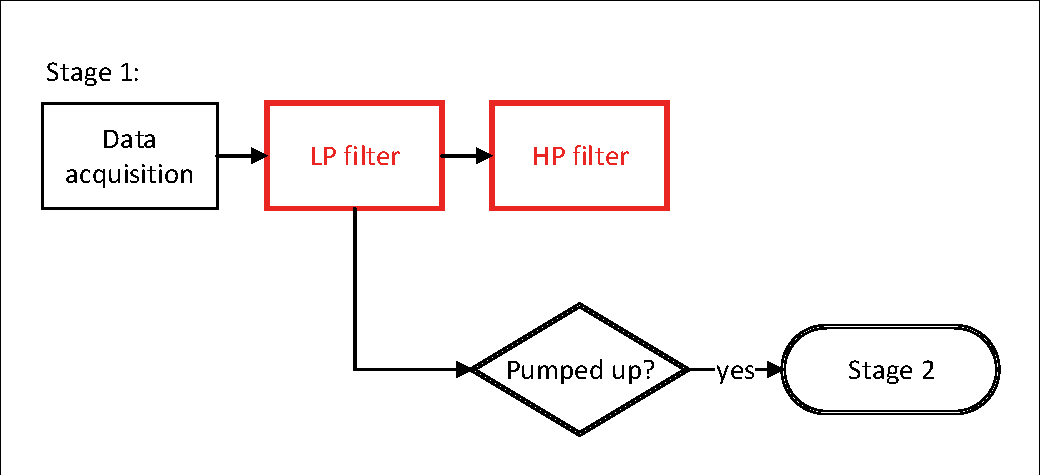
\includegraphics[width=0.7\textwidth]{figures/stage1.pdf}
\caption{The simple basic data processing flow. The data is acquired and passed first to a low-pass filter (\SI{10}{\Hz}) and then to a high-pass filter (\SI{0.5}{\Hz}), resulting in a bandpass output. The first stage of the data processing only checks, if the pressure in the cuff is high enough to start deflation (stage 2).}
\label{fig:stage1}
\end{figure}

\section{Deflation}\label{sec:Deflation}
Figure \ref{fig:algoExplain} shows data recorded during the deflation stage. \circled{1} shows the low pass filtered data which is used in the core algorithm as a reference. \circled{2} is the BP filtered data upon which the algorithm is performed. 

\begin{figure}[ht]
\centering
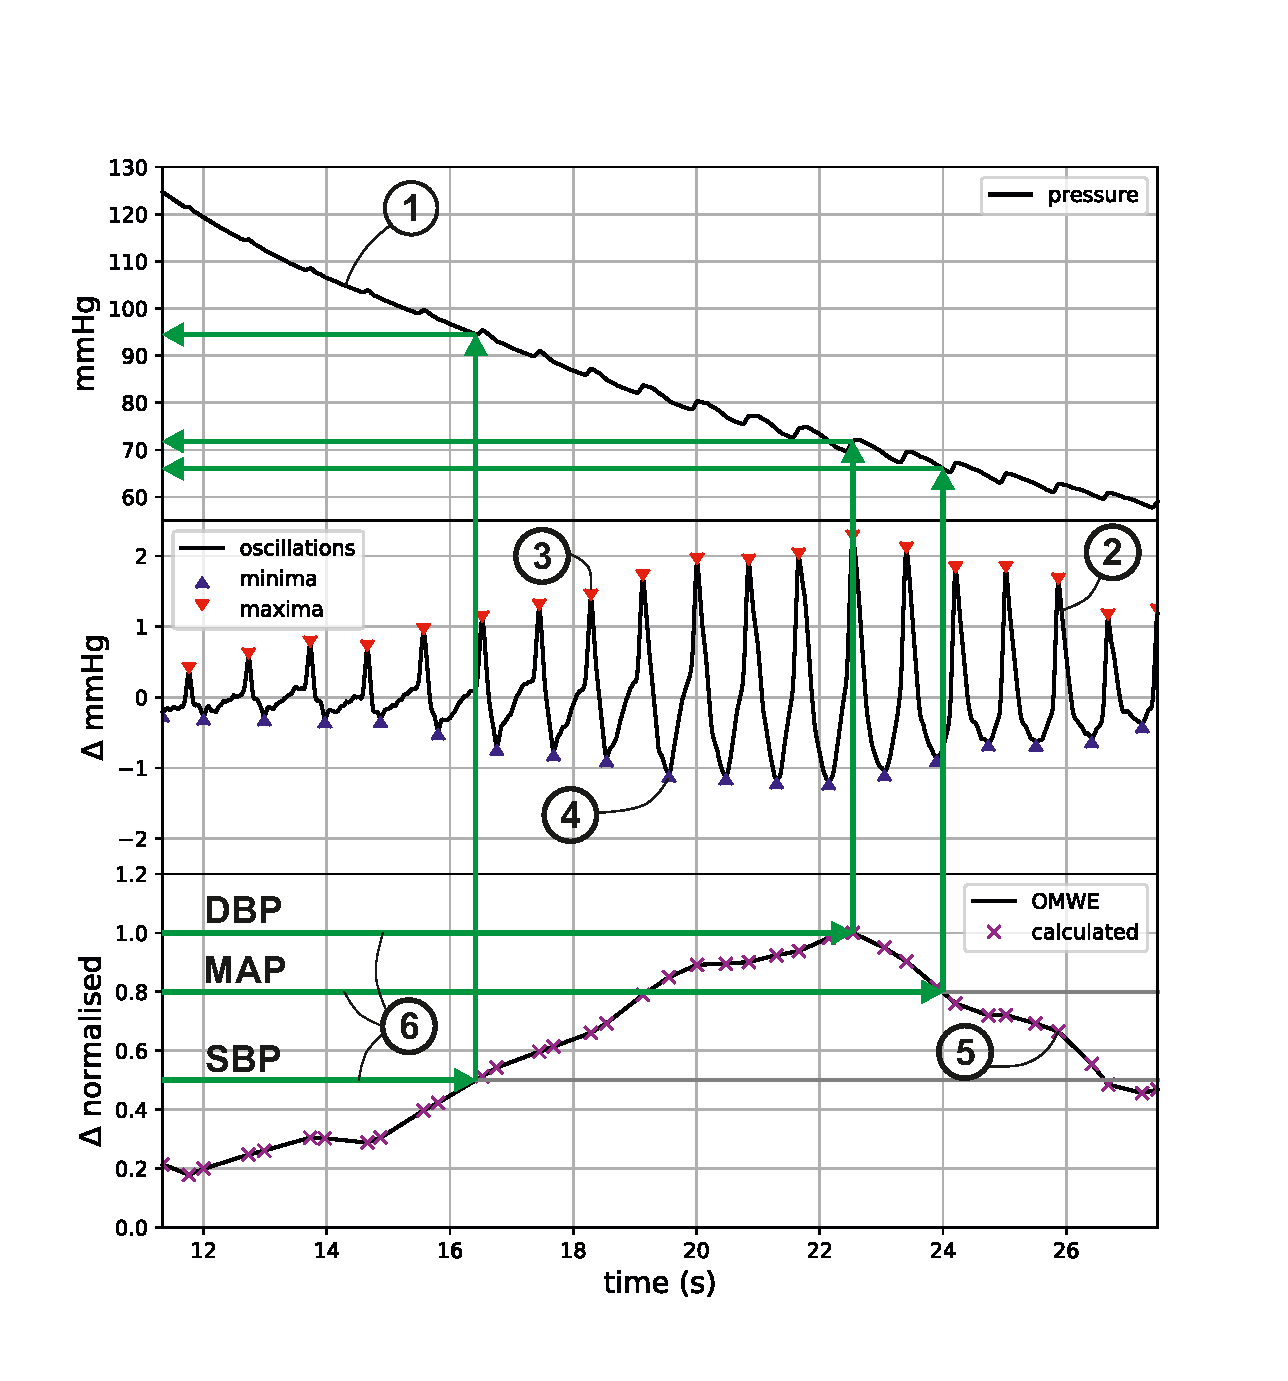
\includegraphics[width=0.95\textwidth]{figures/algorithm_example_annotated.pdf}
\caption{Algo explanation.}
\label{fig:algoExplain}
\end{figure}



\subsection{Extrema Detection}
\paragraph{Maxima}The next step, indicated with \circled{3} is to detect the maxima. Looking at the oscillations, there are local maxima in the troughs between two oscillations. To avoid detecting these, a value needs to have a minimal pronunciation of \SI{0.25}{\Delta\mmHg} to even be considered as a maxima. This limits how the quickly the first oscillations can be detected, but does not influence the algorithm because they are less than \SI{10}{\percent} of the expected maximal amplitude.

A sample is identified as a local maxima, due to the previous and following value being lower. Next, is checked if the current and last detected maxima result in a valid heart rate given by a configurable range. The default range is \SIrange{50}{100}{beats/\minute}. In addition, if the last maxima was less than \SI{300}{\milli\second} ago, only the larger of the two is kept and the lower is discarded.

This is due to two factors that were observed in the data and are shown if figure \ref{fig:maxDetectIssue}. The first, shown on the left hand side, is if the bump in the rising edge of the oscillations results in a detected maxima. This is likely due to artefacts from movement. When oscillations are small and rising, these can lead to wrong detections. This is either irrelevant because they occur before systolic BP or they will be discarded because they lead to errors. 

The second issue is shown in figure \ref{fig:maxDetectIssue} on the right. It occurs mainly when oscillations are decreasing and if the filtering is not optimal. 
\paragraph{Minima} Minima detection, indicated by \circled{4} in figure \ref{fig:algoExplain}, is considerably more difficult, especially in the beginning of oscillations as shown in figure \ref{fig:oscMini}. Because there has to be a minima in between two maxima, minima detection is simplified. After detecting two maxima, the lowest value between them is recorded as the minima.


\subsection{Heart Rate Detection}\label{sec:HR}
Heart rate is already part of the extrema detection described above. Therefore, the current heart rate is detected after each valid maxima starting from the second one. Because each pulse stems from a heart beat, each maxima represents one. By calculating the time between the last two maxima, a heart beat is estimated using equation \ref{eq:HR} below.

\begin{equation}
\label{eq:HR}
pulse=\frac{60s}{t_{curMax} - t_{lastMax}}
\end{equation}

After finishing the measurement, the average heart rate is calculated from all validly detected maxima.


\section{Oscillometric Waveform Envelope}
When the detected maxima, marked by the red triangles in \ref{fig:algoExplain}, have reached their highest amplitude and declined again the oscillometric waveform envelope (OMWE) can be calculated. 

This condition is estimated by taking the largest recorded maximum and multiplying it with the ratio for the diastolic blood pressure minus a hysteresis of $0.3$ (equation \ref{eq:cutoff}. If the last recorded maxima is below this value, the extrema detection part of the algorithm (\circled{3} and \circled{4} in figure \ref{fig:algoExplain}) can be concluded. To avoid a wrong detection of this condition the largest maxima needs to be at least \SI{1.5}{\delta\mmHg}. Otherwise the condition can be detected when oscillations first start occurring and are small with large variations. 

\begin{equation}
\label{eq:cutoff}
A_{cutoff}=A_{Max}\times (r_{DBP} - 0.3)
\end{equation}

\subsection{OMWE Calculation}
To calculate the OMWE from the determined extrema, the following approaches were tested:

\begin{enumerate}[noitemsep]
\item Only considering the maxima.
\item Subtracting the following minimum from each maxima.
\item Subtracting the preceding minimum from each maxima.
\item Interpolating between maxima and minima to find the corresponding values and subtracting them. 
\end{enumerate}

1. works decently, but discards the information in the minima. 2. works well for pressure in the systolic range, because minima follow quickly after maxima. Vice versa, 3. works well in the diastolic range. 4. requires the most computations, but is the least sensitive to noise, because it takes the time difference between minima and maxima into consideration. 

When referring back to figure \ref{fig:algoExplain}, \circled{5} shows how the OMWE was calculated using the \nth{4}approach and calculating a value for each of the maxima and minima separately. 

Figure \ref{fig:interpol} shows how interpolation is used to calculate an interpolated maximum at the time where a minimum occurs to then be able to subtract the minimum from the maximum. Inversely, A minimum is interpolated between two measured minima where a maximum occurs. The resulting plot is displayed in figure \ref{fig:algoExplain} at the bottom. Note that the values are normalised by the maximal value.


\subsection{Determination of Blood Pressure Values}
After calculating the OMWE, the last step is to determine the BP values from it. As explained in chapter \myref{cp:theory}, MAP occurs where the OMWE has its maximum. The time, when the maximum is recorded, is compared to the pressure at that time as indicated by \circled{6} in figure \ref{fig:algoExplain}. To account for the oscillations in the deflation curve, the pressure value is averaged over the period of an average heart beat centred around the detected time. The average heart beat is determined from the measurement as explained in section \myref{sec:HR}. In the example above, this results in MAP of \SI{71}{\mmHg}.

Likewise, to determine SBP and DBP, the specific ratios of the maximal oscillations are searched in the OMWE. The example in figure \ref{fig:algoExplain} uses a ratio for systolic BP of 0.5 and for diastolic BP of 0.8 for simplicity.

The systolic BP is determined by stepping backwards in time from the maximal oscillations and the diastolic BP by stepping forwards in time, respectively. Once the value falls below the specific ratio, interpolation is used to find the time where the exact ratio would have occurred. Using the same approach as for the MAP, the specific values found with \circled{6} for the data in figure \ref{fig:algoExplain} is \SI{95}{\mmHg} for SBP and \SI{67}{\mmHg} for DBP.

%TODO results?
\subsubsection{Implications of Filter Delays}\label{sec:impfilt}
As pointed out in section \myref{sec:filt}, the original data is delayed by first the LP and then the HP filter. Since the oscillogram is based on the LP filtered data, the delay of the first filter (LP) is irrelevant. The second filter (HP) has up to \SI{125}{\milli\second} delay for certain frequencies. Figure \ref{fig:algoDetail} shows the oscillations superimposed over the deflating data. At a deflation rate of \SI{3}{\mmHg/\second}, the error could be \SI{0.375}{\mmHg}. The calculated pressure is averaged over the period of an average heart rate to account for the oscillations in the deflating data and compared to the inaccuracies of the algorithm in general, this is neglectable. 


\begin{figure}[ht]
\centering
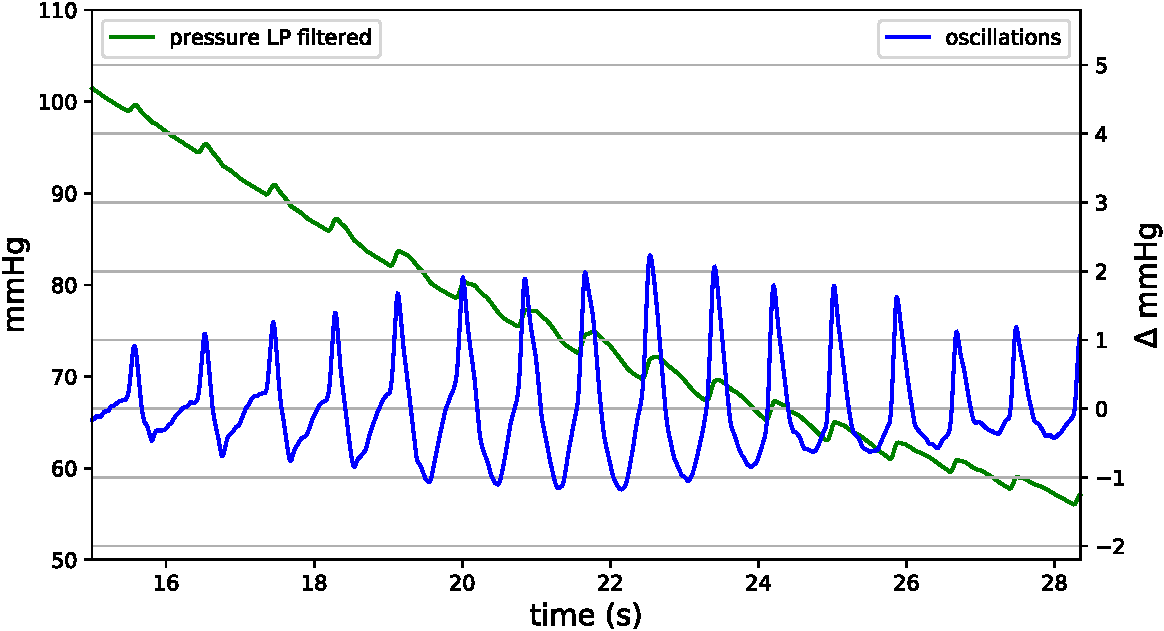
\includegraphics[width=\textwidth]{figures/algo_detail.pdf}
\caption{Algo explanation.}
\label{fig:algoDetail}
\end{figure}

\chapter{Hardware}\label{cp:hw}
This chapter describes the hardware used in this project.

\chapter{Software}\label{cp:sw}

This chapter is a description of the developed software. It provides an overview of the architecture and algorithm implementations. The projects GitHub page provides the full source code, setup instructions and Doxygen documentation \citep{Belinda2020}. %TODO: possibly attach the whole Doxygen documentation (latex format) in attachments"

The project is licensed under the GNU General Public License v2.0.

\section{Overview}
The application is split into the user interface (UI) and data processing. Each part runs in a thread and they are kept separated from each other. The data processing class is called \mintinline{cpp}{Processing} and the user interface class \mintinline{cpp}{Window}. 

The user interface is built with Qt, an open-source widget toolkit for creating graphical user interfaces. Additionally, the subset Qt Widgets for Technical Applications (Qwt) is used to display plots of the acquired data.

The \mintinline{cpp}{Processing} class handles data acquisition and processing, sending notifications to the observer with instructions on what action to perform or what values to update.

\subsection{Class Diagram}
Figure \ref{fig:CD} shows a simplified class diagram of the application. It shows the Processing and Window classes in the middle with their most important attributes. 

The Processing class has a ComediHandler object to acquire data, the OBPDetection object implements the main part of the algorithm and the Datarecord object saves the rawData into a file. 

The Window class holds all the UI components. The class diagram in figure \ref{fig:CD} only shows the high level components that are not directly from the Qt library. SettingsDialog and InfoDialog can be opened through the menu bar to access the configuration and further information about the application. The two Plot objects are always visible, while the rest of the main window depends on the Screen enum.

\begin{figure}[ht]
\centering
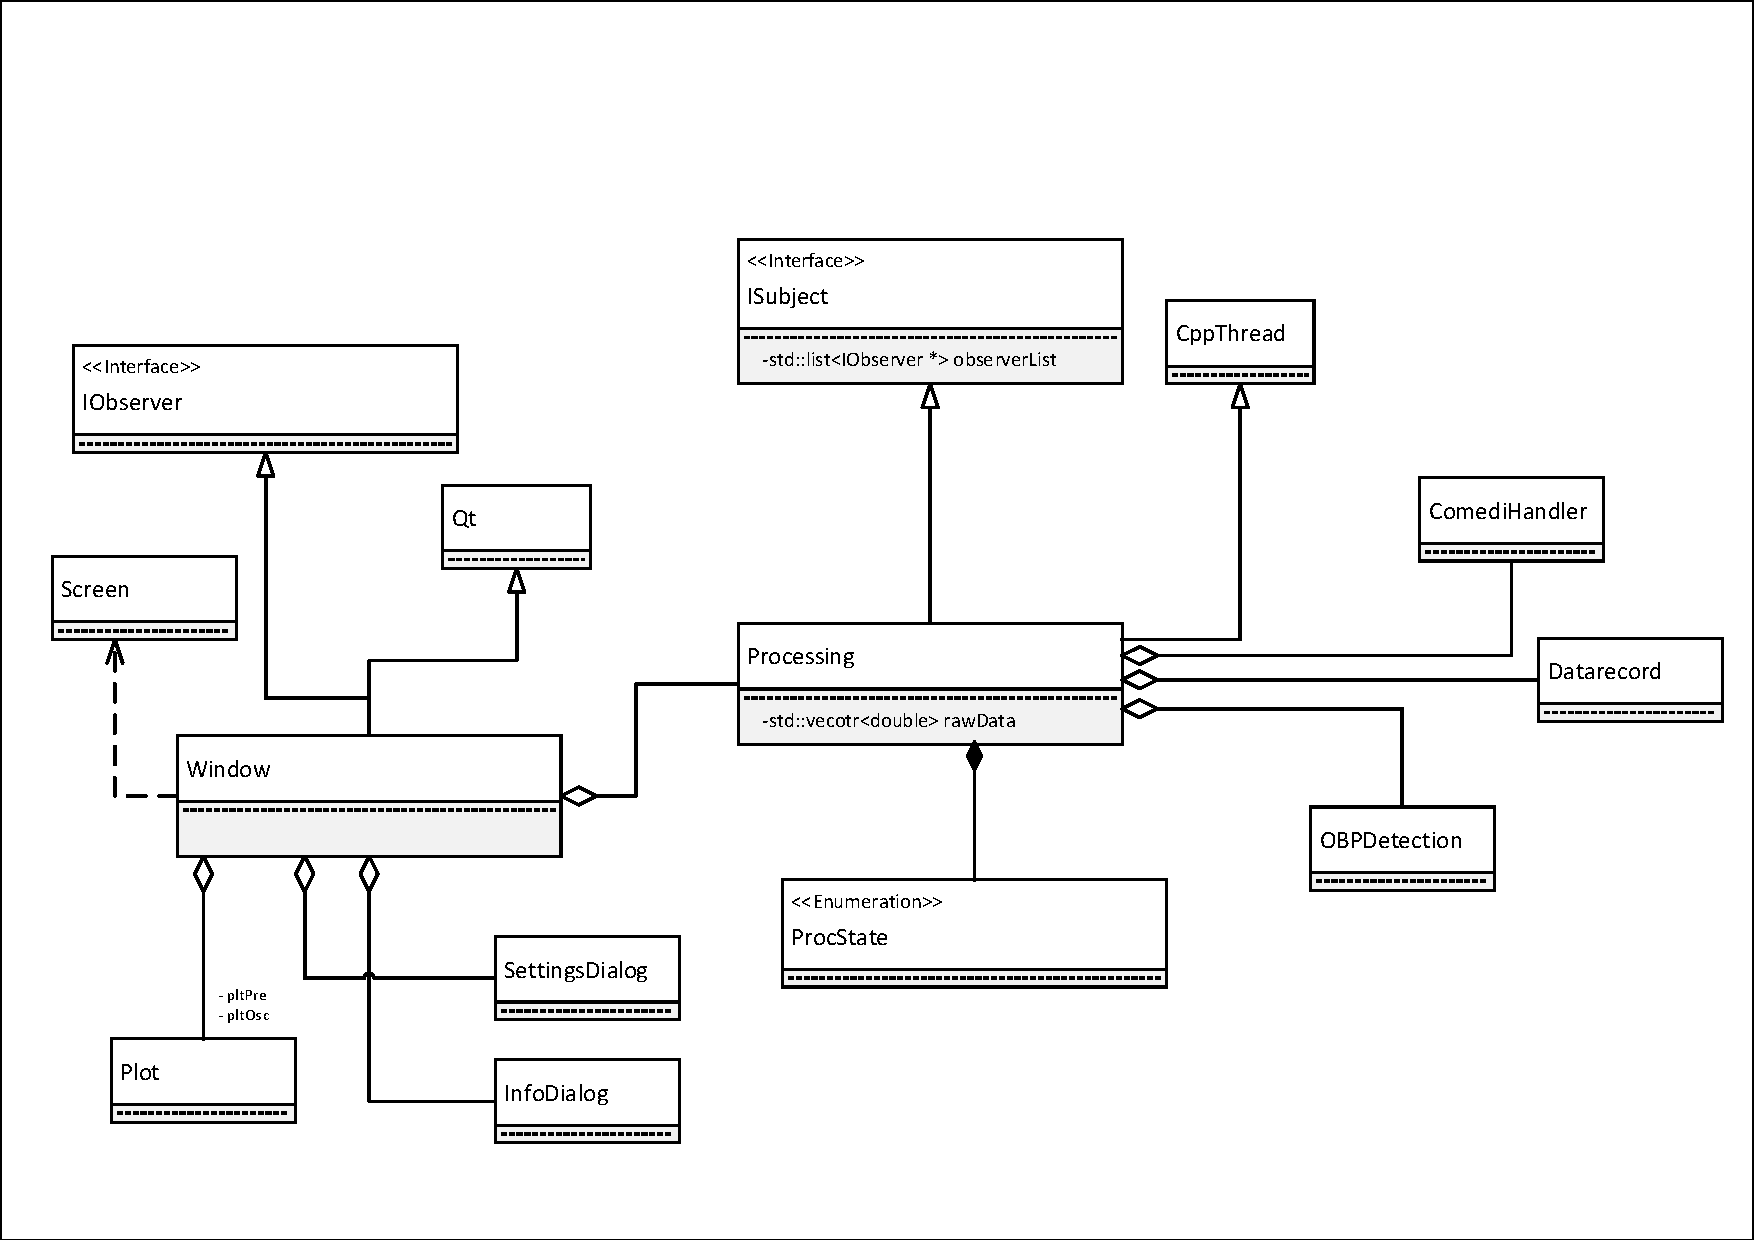
\includegraphics[width=\textwidth]{figures/cd2.pdf}
\caption{The Class Diagram. Needs work.}
\label{fig:CD}
\end{figure}

Communication between the  two main objects is done with callbacks in an observer pattern from the \mintinline{cpp}{Processing} to the \mintinline{cpp}{Window} class. The processing class is an observable subject that the window class can register to because it implements IObserver. The window has a reference to the processing class to pass on user input.

Following is a more in-depth discussion of its elements.

\section{Data Processing}
In the processing class, the data is acquired and processed. The acquisition is handled by a ComediHandler object, that abstracts handling of the underlying hardware. The data is then filtered and the observers are notified so they can display the new data. 

The logic in the processing object is handled through a state machine. The OBPDetection class needs deflating pressure to extract the blood pressure characteristics from the oscillations. The state machine identifies this in the state 'Defalte'. The following section discusses the state machine in detail.

\subsection{State Machine}
Figure \ref{fig:sm} shows the state machine of the processing class. It is made up of one initial state (Config) that is only entered at start-up, an 'Idle' state and four states that are consecutively entered in an ideal measurement, called 'Inflate', 'Deflate', 'Empty' and 'Results'.

For every arriving sample, the state machine is executed according to the current state and potentially switched to another one. 

In every state, exept 'Confi' the arriving sample is filtered and the results are sent to the observing objects. In the Inflate, Deflate and Empty states, the raw data is additionally recorded an ultimately saved as a file when exiting the Empty state. 

\paragraph{Config} After a reset, the state machine starts in the Config state, where the ambient voltage is registered. This is necessary, because the pressure sensor gives an absolute value, but pressure values are needed relative to atmospheric pressure. The raw pressure is read for \SI{250}{ms} and averaged. If that value has a deviation of less than \SI{1}{\milli\volt}, it is stored as ambient pressure and the state machine processes to the next state.

\begin{figure}[ht]
\centering
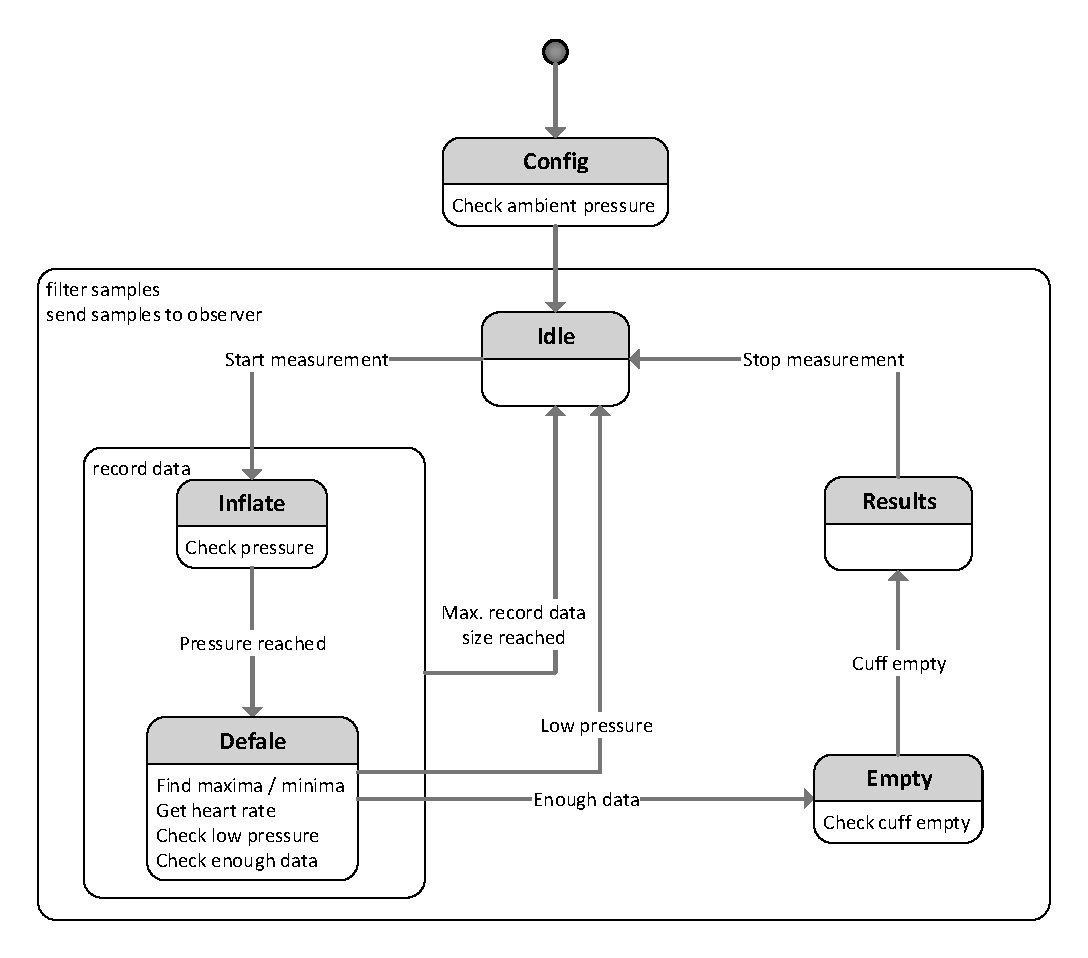
\includegraphics[width=\textwidth]{figures/state_machine.pdf}
\caption{The state machine implemented in the Processing class. Needs work.}
\label{fig:sm}
\end{figure}

\subsection{Processing Class} 
The processing class inherits from the CppThread class and the ISubject class. CppThread is a wrapper to the std::thread class that was written by Bernd Porr to avoid static methods and makes the class a runnable thread. It has an instance of ComediHandler to acquire and two filter instances to pre-process the data. The raw, unfiltered data is sored in a vector that can be handed to the Datarecord instance to save it as a file. Meanwhile, the filtered data is sent to the GUI to display and handed to the OPDetection instance that performs the algorithm. While the data acquisition and filtering are running whenever the thread is running, the state machine described above decides when data is passed to the OBPDetection or stored to a file. 

\subsubsection{Thread Safety}
The processing class has public getter and setter methods, that allow objects, with access to it, to read and change configuration variables. These variables are defined as atomic, to make access to them thread-safe. Similarly, the booleans set by starting and stopping the measurement and stopping the thread are atomic.

\subsection{ISubject}
ISubject is a simple interface that lets the implementing class easily notify its observers about certain events. Each notification is realised as a private notify-X method. The public methods are 'attach' and 'detach'. Through these, a class that implements the above described IObserver (section \ref{sec:iobserver}) can be attached to the subject. This stores a reference to the object in a list. When one of the notify methods is called, the notification is sent to all the observers in the list. The observer can be removed through the detach method. 

Just like the IObserver class, the ISubject class can not be instantiated directly but has to be used to inherit from. 


\subsection{Data Acquisition}

\subsection{Filtering}

\subsection{OBPDetection}

\subsection{Storing the Recorded Data}
%
%\subsection{Project Setup and Compilation}
%The project is set up as a CMake project. Usually, Qt projects are set up using qmake (a .pro file), but CMake is supported as well. This application chose CMake because it is more powerful and allows integration with other tools, e.g. for continuous integration (CI). %TODO potentially include information about Travis CI (if set up)
%
%CMake ensures all required dependencies are installed as defined in the file CMakeList.txt and automatically generates a Makefile. This Makefile is used to build the project, linking all defined files and libraries.
%For example, this application requires the C++20 standard for the implemented algorithm. CMake generates an error when trying to build the application with a compiler that does not support C++20.



\section{User Interface}
The user interface is shown in figure \myref{fig:UI}. It is split up into two parts. The left side accepts user input and gives instructions to the user what they have to do to take their blood pressure. The right side shows the data being acquired in real-time. There are two plots. The upper plot shows pressure data filtered with a low-pass filter of \SI{10}{\Hz}, the lower plot shows the data additionally low-pass filtered at \SI{0.5}{\Hz}, which results in a bandpass filter. This is the oscillogram that is the main input for the algorithm to determine the user's blood pressure.

\begin{figure}
\centering
%
\includegraphics[scale=0.125]{GlaLogo.pdf}
\caption{UI}
\label{fig:UI}
\end{figure}

As mentioned above, the graphical user interface (GUI) is built with Qt.
The QtDesigner was used to design a first draft of the GUI, but because this does not allow integration into applications that are built outside of the Qt development environment, the whole GUI was completely built-in C++ code from this draft.

\subsection{Guided Blood Pressure Measurement}
The left side of the GUI guides the user through taking blood pressure. The process is split up into five pages that are shown in figure \ref{fig:UIguide}.  All pages have a dial that shows the current pressure in \SI{}{\mmHg}. The first page has information on how to prepare for the measurement. Pressing the button at the bottom of the page starts the measurement process. The button is only enabled if the processing part of the application is ready.

\begin{figure}[ht]
\centering
%
\includegraphics[scale=0.125]{GlaLogo.pdf}
\caption{The screens that guide the user through taking their blood pressure in the order that they are shown.}
\label{fig:UIguide}
\end{figure}

The second page instructs the user to pump up the pressure in the cuff to a certain value. The default value is \SI{180}{\mmHg}. Once that value is reached, the GUI automatically switches to the next page.

This page tells the user to release the pressure in the cuff again. This should be done slowly at a rate of approximately \SI{3}{\mmHg/\second}. There is currently no other feedback than the dial for how fast the pressure is being released. At the bottom of the page, the current heart rate, calculated from the latest oscillation peaks, is shown.

Once enough data is collected, the fourth page is shown. It requires the user to deflate the cuff completely to show the results. If the algorithm fails to collect enough data within a specified time (currently configured as 5 minutes) the measurement stops and goes back to the start page.

When the pressure in the cuff reaches nearly zero, the final results page is shown. It displays MAP, SBP, DBP and the average heart rate during the measurement. All data is shown as whole numbers without decimals. 

\subsection{Menu}
A menubar provides access to an information pane as well as a settings pane. Both open up as dialogue windows and disable user input on the main window. Data acquisition is kept running and is displayed in the plots.

\subsubsection{Information}
The information pane shows the application version number, shows the licence and provides a link to the project GitHub page. Figure \ref{fig:UIinfo} shows the dialogue.

\begin{figure}[ht]
\centering
%
\includegraphics[scale=0.125]{GlaLogo.pdf}
\caption{The information dialogue.}
\label{fig:UIinfo}
\end{figure}


\subsubsection{Settings}
The settings dialogue (shown in figure \ref{fig:UIsettings}) lets the user change some application configurations. The user is not recommended to change these if they are not aware of the consequences. The settings are stored persistently but only take effect after restarting the application. The range of accepted values is limited, to keep the algorithm working. Because not all values have been tested, the user is warned that the application might not perform reliably anymore. The values are stored once the user presses the 'OK' button. If the 'Cancel' button is clicked, the settings application closed without saving the values.

The values can be reset by pushing the corresponding button. These changes take effect immediately. 

\begin{figure}[ht]
\centering
%
\includegraphics[scale=0.125]{GlaLogo.pdf}
\caption{The settings dialogue.}
\label{fig:UIsettings}
\end{figure}

The handling and storing of these values are done through the QSettings class of the Qt library. It allows to save and load values by specifying a string key. If there is no key found with the provided key, the default value is selected. The default value is what is hardcoded in the Processing class.

\subsection{The Window Class}
The \mintinline{cpp}{Window} class inherits from the \mintinline{cpp}{QMainWindow} class and the \mintinline{cpp}{IObserver} class. The \mintinline{cpp}{QMainWindow} class makes the class an executable Qt window, with Qt taking care of updating the GUI and generating events for button clicks and so on. The \mintinline{cpp}{IObserver} makes the class able to be registered as an observer for a subject that will send notifications to the observer. More on the \mintinline{cpp}{IObserver} below.

All GUI elements are set up in the constructor of  \mintinline{cpp}{Window}, including the settings and info plane. However, they will only be shown if necessary. E.g. what page of the user instructions is shown is defined by the setting of the screen enum (currentScreen).

The Window object is instantiated with a reference to a Processing object in the constructor. This is necessary so the user inputs can be relayed and the Processing thread can be stopped when the window is closed and the application exited. 

\subsection{The IObserver Class}
The \mintinline{cpp}{IObserver} class defines the functions that the observable class (the subject) uses to notify the observer. All functions are virtual but implemented as empty functions. This way, the observing class can choose to implement and therefore listen to the notifications that it wants to and ignore the ones that it does not. 

The IObserver class can not be instantiated directly but has to be used to inherit from. This is achieved by having a protected constructor.

\paragraph{The following methods can be implemented:}
\setlist{nolistsep}
\begin{itemize}[noitemsep]
\item Ready: \newline
Informs the observer that the subject is ready.
\item New Data: \newline
Sends a new data pair to the observer. Each data pair consists of pressure data and oscillation data. Both are doubles.
\item Switch Screen: \newline
Tells the observer which screen to display.
\item Results: \newline
Sends the results to the observer. The results are three doubles for MAP, SBP and DBP.
\item Heart Rate: \newline
Sends a new heart rate value to the observer. The value is a double.
\end{itemize}

These methods are called from a class that inherits from ISubject, which is explained in detail in section \ref{sec:isubject} below. 

\subsubsection{Thread safety}
Because the methods from the \mintinline{cpp}{IObserver} class are called from an object, which is likely to be running in another thread than the window, it is important to implement all functions in a thread-safe manner. Qt offers a good way to do this by sending queued events. 

One example of how to enable the start button, in a not thread-safe way is by accessing it directly, as follows: 

\begin{minted}[breaklines]{cpp}  
btnStart->setDisabled(false);
\end{minted}

Instead, the function \mintinline{cpp}{QMetaObject::invokeMethod} is called to send an event to the GUI thread. This is done by specifying the object, which function of the object to call, what arguments to set, and the type of event to send. The \mintinline{cpp}{Qt::QueuedConnection} will send an event into a queue that will be handled when the thread is executed. The function to call is given as a string argument. Considering the example above, this results in the following statement:

\begin{minted}[breaklines]{cpp}  
bool bOk = QMetaObject::invokeMethod(btnStart, "setDisabled", Qt::QueuedConnection,  Q_ARG(bool, false));
assert(bOk);
\end{minted}

The return value confirms if the connection could be made, i.e. the given string is a valid function to call for the given object. This is tested through an assert during development. The assert will fail if the boolean is not true. It is important not to have the assert around the whole function call, because it will be removed in the release build. 

The plots have their underlying data set changed every time a new sample is available because a new sample is always added on the right side and an old one is discarded on the left side. This is made by changing the raw data in memory and therefore, the Qt process is not informed about that. To solve this issue, the plots are regularly updated manually. This happens in a timer event with an interval of 50 ms, which is enough for the human eye to see a continuous movement. To avoid thread safety problems, the plot objects are accessed after acquiring a mutex.


%TODO \section{Settings}
\section{Third Party Software}

\begin{itemize}
\item Qt %TODO ref
\item CppThread a wrapper to the std::thread class written by Bernd Porr to avoid static methods. %TODO ref
\item \emph{iir1} An implementation of the infinite impulse response (IIR) filters for sample-by-sample, real-time processing written in C++ by Bernd Porr. Provided as a library.%TODO ref
\item \emph{plog} Portable, simple and extensible C++ logging library. %TODO ref
\end{itemize}


\chapter{Results and Discussion}\label{cp:res}

The goal of this project was to be able to conduct experiments with test subjects and to record datasets. Unfortunately, due to the ongoing situation when this project was conducted, this was not possible. Even though all possible safety measurements were considered and approved by the University's risk assessment department, the approval process was rendered impossible to go through within the given time frame. Apart from not being able to record any datasets, the algorithm might suffer from systematic errors due to subjective charasteristics in the developers blood pressure oscillations. 


This chapter highlights important results of the project.


- valve needs to open continuously to have a steady stream of 3mmHg/s
  opening introduces noise

- many algorithms only work for clean data

- MAP is used for diagnostics 

\chapter{Conclusion} %TODO probably redundant to results?

This chapter discusses the outcome of the project and proposes the next steps to take.

%ry not to mention "IT"

%Testing on human subjects other than the developer could not take place due to the situation at the time of writing. A concept for testing was introduced and approved by the risk assessment department, however, the ethics application could not be resolved with the situation making the application process impossible to go through in the short period of time that this thesis was written.


The goal of this project was to be able to conduct experiments with test subjects and to record datasets. Unfortunately, due to the ongoing situation when this project was conducted, this was not possible. Even though all possible safety measurements were considered and approved by the University's risk assessment department, the approval process was rendered impossible to go through within the given time frame. Apart from not being able to record any datasets, the algorithm might suffer from systematic errors due to subjective charasteristics in the developers blood pressure oscillations. 

%Everyreportmusthaveconclusions,builtonthediscussion.Thissectionincludesasummaryofthemainachievementsoftheworkbutismorethanthat. Thenoun‘conclusion’canbedefinedas‘ajudgementordecisionreachedbyreasoning’[8]soyoushouldhighlightwhathasbeenlearntasaresultofyourproject.Whatisthebigpicturethatthereadershouldtakeaway?TheConclusionsshouldincludeanassessmentoftheoutcomeagainsttheoriginalaimsoftheproject.Ifyouwereunabletofulfilsomeaims,explainwhy. Itisalsousefultore-viewtheprojectplan(whichshould beincludedwiththereport).Didsometasksprovetobeunexpectedlydifficult,for instance?


%TODO further steps:
% check that in defaltion, it is actually defalting
% give feedback for deflation speed


% highly dependant on noise for SBP and DBP because of the way it is calculated
%oscillometry good for MAP, rest should be done by sounds
% challenge: how to make sure you can hear sound
% and the other chapters
\appendix
%\chapter{Derivation of the equation}

This is such boring material that it has been relegated to an appendix. Let's check an equation:
\begin{equation}
x = \frac{-b \pm \sqrt{b^2 - 4ac}}{2a} .
\label{quadratic soln}
\end{equation}
Let's hope I got it correct.


\backmatter  % Turn off chapter numbering
%\bibliographystyle{IEEEtran}
\bibliographystyle{plainnat}%{agsm}{apa}
\bibliography{references}
%TODO update all references!!!

\end{document}
